\chapter{Theory} 
\label{ch:theory}

\minitoc

%What's the standard model all about? 

%\section{In the beginning...}
%\section{Some other stuff}



%\section{The Standard model of Particle of Physics}
\section{The weak force in \bquark-hadron decays}

Ground state \bquark-hadrons can only decay via the weak interaction as the \bquark-quark must change flavour to one of the first or second generation quarks.
Exclusive decays of \B mesons were first observed by the \cleo experiment in 1983~\cite{PhysRevLett.50.881}. Although the weak interaction dictates the core of the process, the contributions from the strong force are unavoidable. In the SM quarks abide by \emph{confinement}, preventing bare quarks from propagating unhindered. Instead quarks are only ever observed in bound states, or hadrons, with other quarks or anti-quarks. Therefore the observation of the weakly decaying \bquark-quark is necessarily accompanied by the strong interaction governing the hadronisation of the initial and final state quarks.


\subsection{The weak force}

The weak interaction differs remarkably from the electromagnetic and strong interactions. It is the only of the three to be mediated by massive gauge bosons and uniquely violates parity; the action of mirroring space. 
Additionally, there are two types of gauge boson: the charged \Wpm bosons that result in \emph{charged-current} interactions; and the neutral \Z boson, responsible for \emph{neutral-current} interactions. 

Confusingly, the weak interaction is actually stronger than the electromagnetic force, however the large mass of the mediators suppresses the interaction at low energy.
The \emph{charged-current} weak interaction was originally described by Fermi using a four point coupling $G_{\text{F}}$. 
%This was introduced to account for the missing energy taken away 
This works well for low energy interactions in which the momentum transfer is much less than the \Wpm boson mass, $|q^{2}|<<m_\Wpm^2$. In the higher mass range this breaks down leading to unitarity violation in processes such as \decay{\ep\en}{\Wp\Wm}. This is resolved by the addition of the neutral \Z boson and the \emph{neutral-current} interactions that restore unitarity. 


\subsubsection{Parity violation}
Parity is conserved in QCD and QED so it was naturally assumed to follow suit in the weak interaction. In 1957 is was shown by C.S. Wu and collaborators that parity was indeed violated in the beta decay of cobalt-60~\cite{PhysRev.105.1413}. The rate of electrons emitted during the decay were measured as a function of the polar angle. In the parity conservation scenario the same rates would have been expected at angles of $\theta$ and $180^\circ-\theta$ to an applied magnetic field; however electrons are preferably emitted against the field.          

The weak interaction can be described as a V-A interaction (vector-axialvector), corresponding to a maximally parity violating interaction; the \Wpm boson only couples to left-handed chiral particle states. In the ultra-relativistic limit this would mean that the weak force only couples to left-handed helicity particles and right-handed helicity antiparticles. {\color{Red} define helicity?} This is relaxed when accounting for the non-zero masses of fermions (when the helicity eigenstates are no longer equal to the chiral eigenstates), but leads to helicity suppression for certain processes, for example \decay{\pim}{\en\neueb} with respect to \decay{\pim}{\mun\neumb}. The relative branching fractions for these two processes acts as strong experimental evidence for the V-A interaction.

\subsubsection{Electroweak unification}

Although the weak and electromagnetic forces can be described by QED and the Fermi interaction at low energies, this becomes insufficient at high energies. Here, the weak and electromagnetic forces can be unified through the single Electroweak gauge theory with a $\text{SU}(2)_{L}\times\text{U}(1)_{Y}$ symmetry.

The \Z boson introduced to prevent unitarity violation is experimentally observed to couple to both left-handed and right-handed particles, in contrast to the \Wpm boson. This seemingly contradictory situation was resolved by Glashow, Salam and Weinberg~\cite{Glashow:1959wxa,Salam:1968rm,Weinberg:1967tq} who developed a unification of the electromagnetic and weak interactions. 
This begins by replacing the physical electromagnetic $\text{U}(1)_{\text{Q}}$ interaction with a similar $\text{U}(1)_{\text{Y}}$ interaction that couples to weak hyper-charge, $Y$. This gauge symmetry requires a new gauge boson $B$. The weak $\text{SU}(2)_{L}$ interaction generates three gauge bosons. The third of these, the neutral $W^{3}$, can mix with the new $B$ gauge boson to generate the two physical bosons $\gamma$ and \Z
\begin{equation}
\left( \begin{array}{c} \gamma \\ \Z \end{array} \right) = \begin{pmatrix} \cos{\theta_{W}} & \sin{\theta_{W}} \\ -\sin{\theta_{W}} & \cos{\theta_{W}} \end{pmatrix} \left( \begin{array}{c} B \\ W^{3} \end{array} \right),
\end{equation}
where $\theta_{W}$ is the weak mixing angle. 
This allows the \Z boson to couple to both left- and right-handed particles as it is a mixture of the parity-violating $\W^{3}$ boson and parity-conserving $B$ boson.  


\subsection{Weak interactions of quarks}


It is experimentally observed that the rates of kaon and pions decays do not proceed at the same rate; the decay rate of \squark-quark containing particles are suppressed,
\begin{equation}
\frac{\Gamma(\decay{\Kp}{\mup\neum})}{\Gamma(\decay{\pip}{\mup\neum})}\sim 0.257.
\end{equation}
It was observed by N. Cabibbo that in many quantum mechanical systems, different \emph{good} quantum numbers are appropriate depending on the dynamics. He proposed that the eigenstates of the weak interaction may be different to the mass eigenstates that govern the propagation of particles~\cite{PhysRevLett.10.531}.
%It was proposed by N. Cabibbo that, as with many other quantum mechanical processes, the eigenstates of the weak interaction may be different to the mass eigenstates that govern the propagation of particles~\cite{PhysRevLett.10.531}. Systems can described by different \emph{good} quantum numbers depending on the dynamics. 
The Cabibbo angle, $\theta_{c}$, was introduced to mix the mass eigenstates into the weakly interacting eigenstate,
\begin{equation}
d' = \cos{\theta_{c}}d + \sin{\theta_{c}}s.
\end{equation}
However, this on its own was not enough to explain the lack of flavour-changing neutral currents such as \decay{\Kz}{\mup\mun}. This was resolved by S.L. Glashow, J. Iliopoulos, and L. Maiani with the introduction of the GIM mechanism~\cite{PhysRevD.2.1285}. This suppressed neutral current processes by proposing a fourth quark, the charm quark. This was paired with the strange quark and allowed  Cabibbo's mixing matrix to be elegantly completed
\begin{equation}
\left( \begin{array}{c} d' \\ s'  \end{array} \right) = \begin{pmatrix} \Vud & \Vus \\ \Vcd & \Vcs \end{pmatrix} \left( \begin{array}{c} d \\ s \end{array} \right)= \begin{pmatrix} \cos{\theta_{c}} & \sin{\theta_{c}} \\ -\sin{\theta_{c}} & \cos{\theta_{c}} \end{pmatrix} \left( \begin{array}{c} d \\ s \end{array} \right).
\end{equation}

In the SM the weak interaction facilitates the changing of quark flavour via the \emph{charged-current} interaction $\decay{\Wpm}{q\bar{q'}}$ whilst the \emph{neutral-current} interaction must conserve flavour, $\decay{\Z}{q\bar{q}}$. 


\subsection{The CKM matrix}
Cabibbo's two-generation mixing matrix can be easily extended to the three-generation scenario in the SM. The extended matrix referred to at the Cabibbo-Koboyashi-Maskawa (CKM) matrix~\cite{CKM} is expressed generally as 
\begin{equation}
\left( \begin{array}{c} d' \\ s'  \\ b' \end{array} \right) = \begin{pmatrix} \Vud & \Vus & \Vub \\ \Vcd & \Vcs & \Vcb  \\ \Vtd & \Vts & \Vtb \end{pmatrix} \left( \begin{array}{c} d \\ s  \\ b \end{array} \right)
\end{equation}
where the transitions between quark flavours are determined by the complex quantities $V_{qq'}$. 
In the SM this matrix is required to be a unitary matrix obeying the condition
\begin{equation}
U_{\text{CKM}}^\dag U_{\text{CKM}} = I.
\end{equation}
Therefore, the extension of the mixing matrix not only allows all three generations to be considered, but also increases the number of terms that parametrise the mixing matrix from one to four. Of these four parameters, three can be represented as angles and one must be interpreted as a complex phase. Importantly, this phase allows \CP violation to be present in the SM and was one of the main motivations of M. Koboyashi and T. Maskawa in proposing the matrix.
The matrix can be represented in the Wolfenstein parametrisation using four parameters $\lambda$, $A$, $\rho$ and $\eta$~\cite{PhysRevLett.51.1945}. When represented with factors up to $\mathcal{O}(\lambda^{3})$, the CKM matrix is given by 
\begin{equation}
\left( \begin{array}{c} d' \\ s'  \\ b' \end{array} \right) = \begin{pmatrix} 1 - \lambda^2/2 & \lambda & A\lambda^3(\rho-i\eta) \\ -\lambda & 1-\lambda^2/2 & A\lambda^2  \\ A\lambda^3(1-\rho-i\eta) & -A\lambda^2 & 1 \end{pmatrix} \left( \begin{array}{c} d \\ s  \\ b \end{array} \right).
\end{equation}
This representation is helpful as it dictates that for \CP violation to be present in the SM, $\eta$ must be non-zero. Additionally, the contribution from the imaginary parts is predominately in \Vub and \Vtd (the terms \Vcd and \Vts receive smaller contributions from $\eta$ at $\mathcal{O}(\lambda^{5})$). 

The magnitudes of the CKM matrix elements can be inferred from various processes and have been measured to have the following sizes~\cite{PDG2016}
\begin{equation} 
    \begin{pmatrix} 
        |\Vud| & |\Vus| & |\Vub| \\ 
        |\Vcd| & |\Vcs| & |\Vcb|  \\
        |\Vtd| & |\Vts| & |\Vtb| 
    \end{pmatrix}
    =
    \begin{pmatrix} 
        0.97417\pm0.00021        & 0.2248\pm0.0006           & (4.09\pm0.39)\times10^{-3}\\ 
        0.220\pm0.005            & 0.995\pm0.016             & (40.5\pm1.5)\times10^{-3} \\
        (8.2\pm0.6)\times10^{-3} & (40.0\pm2.7)\times10^{-3} & 1.009\pm0.031            
    \end{pmatrix}.
\end{equation}
The values of the diagonal elements are determined to be close to unity, with the elements getting smaller further away from the diagonal.

The first observation of \CP violation occurred in 1964 by V. Fitch and J. Cronin~\cite{PhysRevLett.13.138}.  
A beam of long-lived neutral kaons was produced and the decay to $2\pi$ was observed. Neutral kaons were known to decay to $2\pi$ and $3\pi$ final states. The $2\pi$ state is a +1 eigenstate of the \CP operation, whilst the $3\pi$ is a -1 eigenstate. If the long-lived and short-lived neutral kaon eigenstates were also \CP eigenstates then only the $\decay{\KS}{\pi\pi}$ and $\decay{\KL}{\pi\pi\piz}$ decays would be allowed. The observation of \decay{\KL}{\pip\pim} decays demonstrated that the physical kaon states did not conserve \CP symmetry. 

Mesons containing \cquark-quarks have not been observed to violate \CP asymmetry. The SM predictions for \CP violation in the charm sector are very small as a result of the CKM elements that govern these processes.     

% {\color{Red}
% \begin{itemize} 
% \item for pseudo-scalars just change C, for baryons more complicated
% \end{itemize}}

\subsection{\bquark-hadron physics}
Hadrons containing \bquark-quarks are a rich environment to study CKM physics. 
There are a wide variety of topologies that allow different parameters to be measured. 
In the \bquark-meson sector \CP violation has been observed in decays of \Bp~\cite{PhysRevD.82.072004,PhysRevD.81.112002}, \Bz~\cite{PhysRevLett.87.091801,PhysRevLett.87.091802}, \Bs~\cite{PhysRevLett.110.221601} mesons.
Neutral \B mesons are observed to oscillate between the particle and antiparticle states, allowing the extraction of ratios of CKM matrix elements.


{\color{Red}
\begin{itemize}
\item lifetime maybe? 
\end{itemize}}



This thesis is concerned with hadronic two- and three-body decays of charged \B mesons.
The relevant topologies of hadronic two-body \Bp meson decays are shown in Fig.~\ref{fig:Theory_topo}. 
%%%%%%%%%%%%%%%%%%%%%%%%%%%%%%%%%%%%%%%%%%%%%%%%%%%%%%%%%%
\begin{figure}[!h]
    \centering
    \begin{subfigure}[b]{0.32\textwidth}
        \centering
        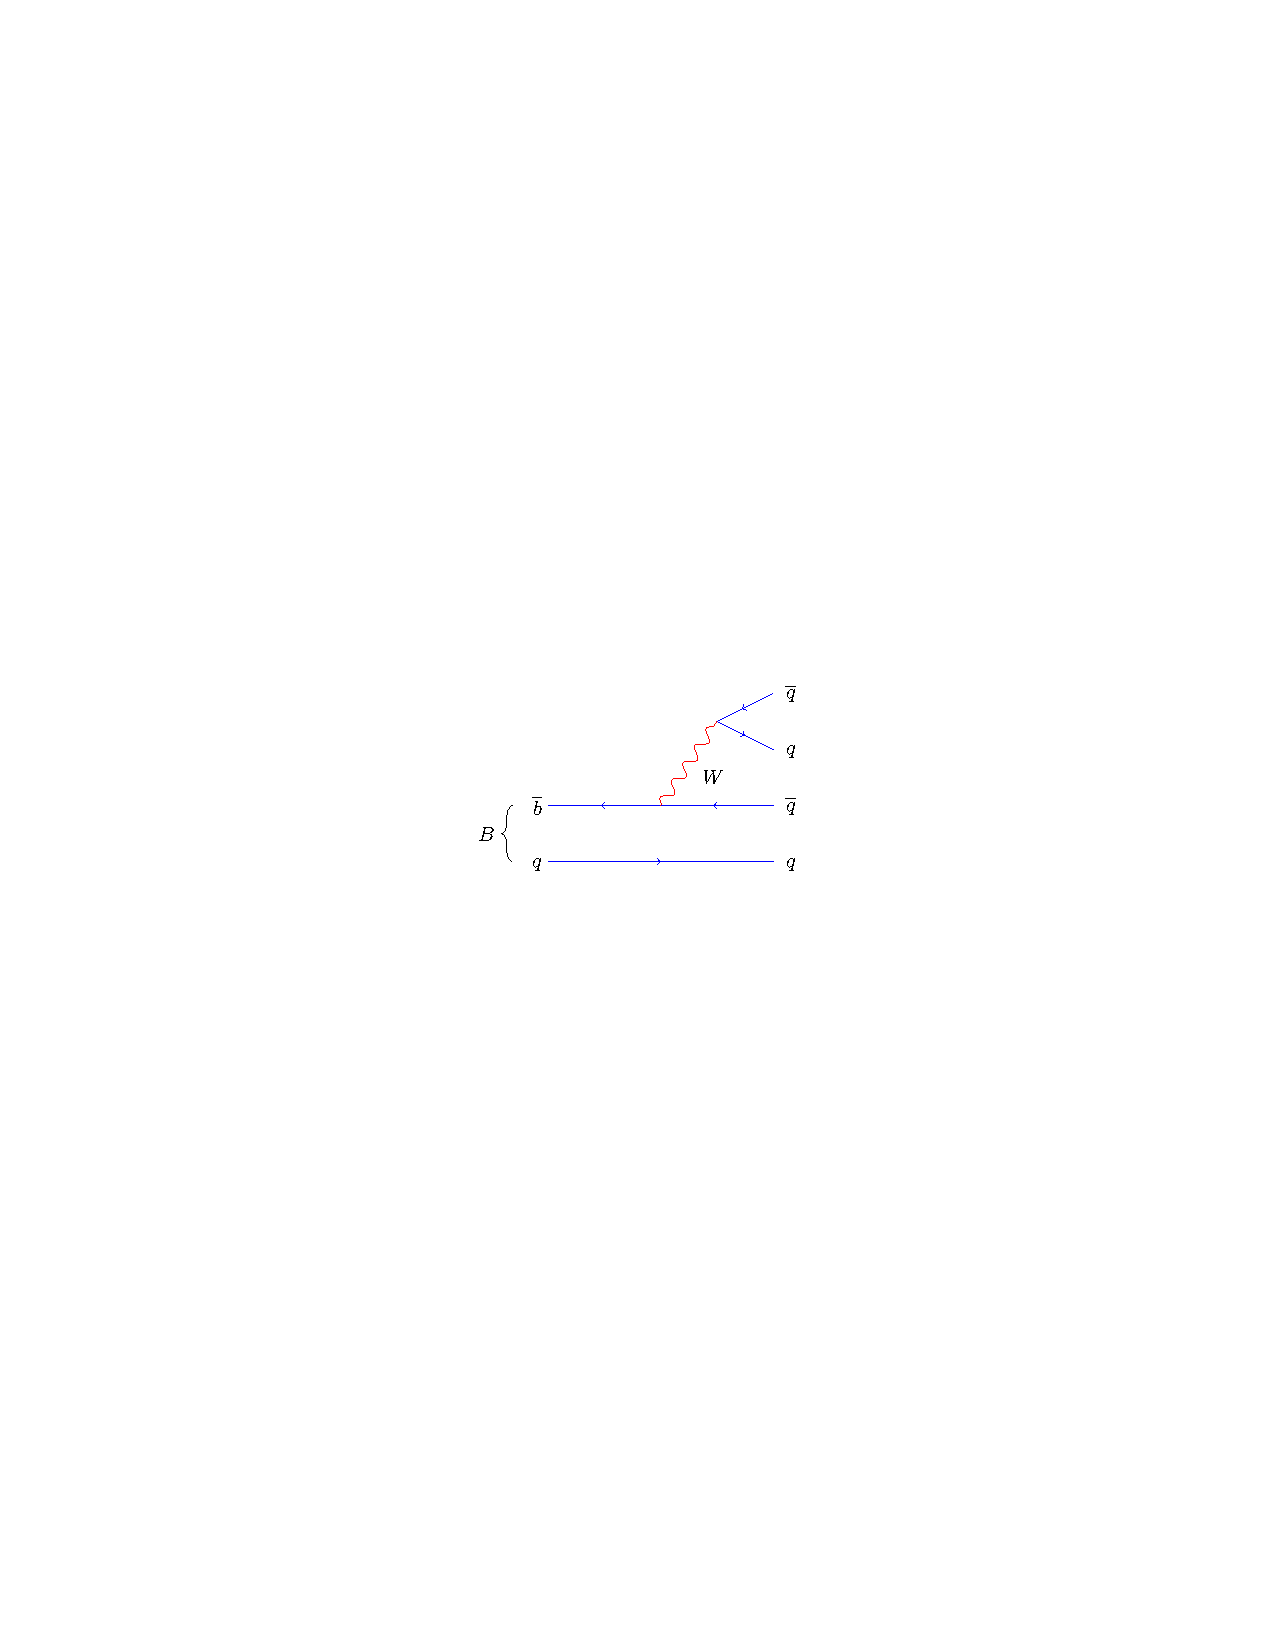
\includegraphics[width=1.0\textwidth]{figs/Theory/TreeFav.pdf}
        \caption{Colour-favoured Tree}
        \label{fig:theory_colour_fav}
    \end{subfigure}
    \begin{subfigure}[b]{0.32\textwidth}
        \centering
        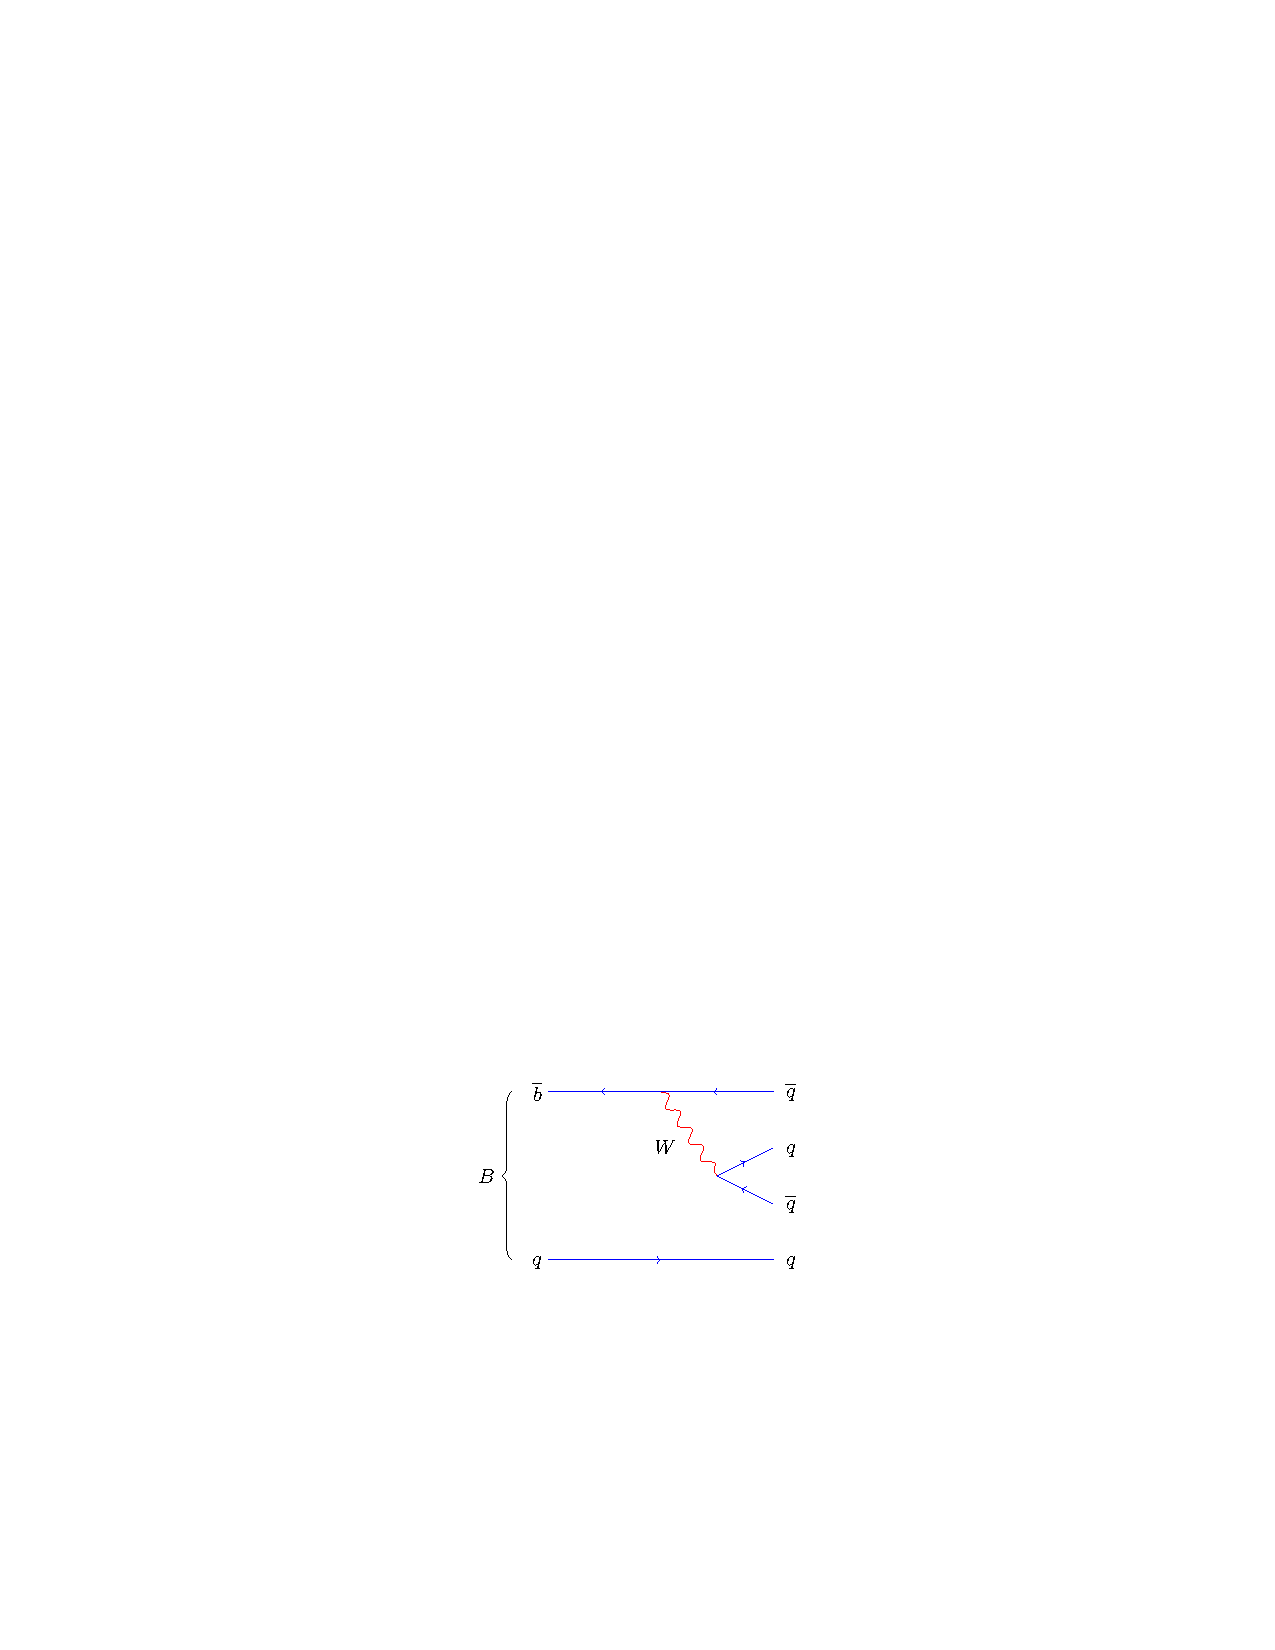
\includegraphics[width=1.0\textwidth]{figs/Theory/TreeSup.pdf}
        \caption{Colour-suppressed Tree}
        \label{fig:theory_colour_sup}
    \end{subfigure}
    \begin{subfigure}[b]{0.32\textwidth}
        \centering
        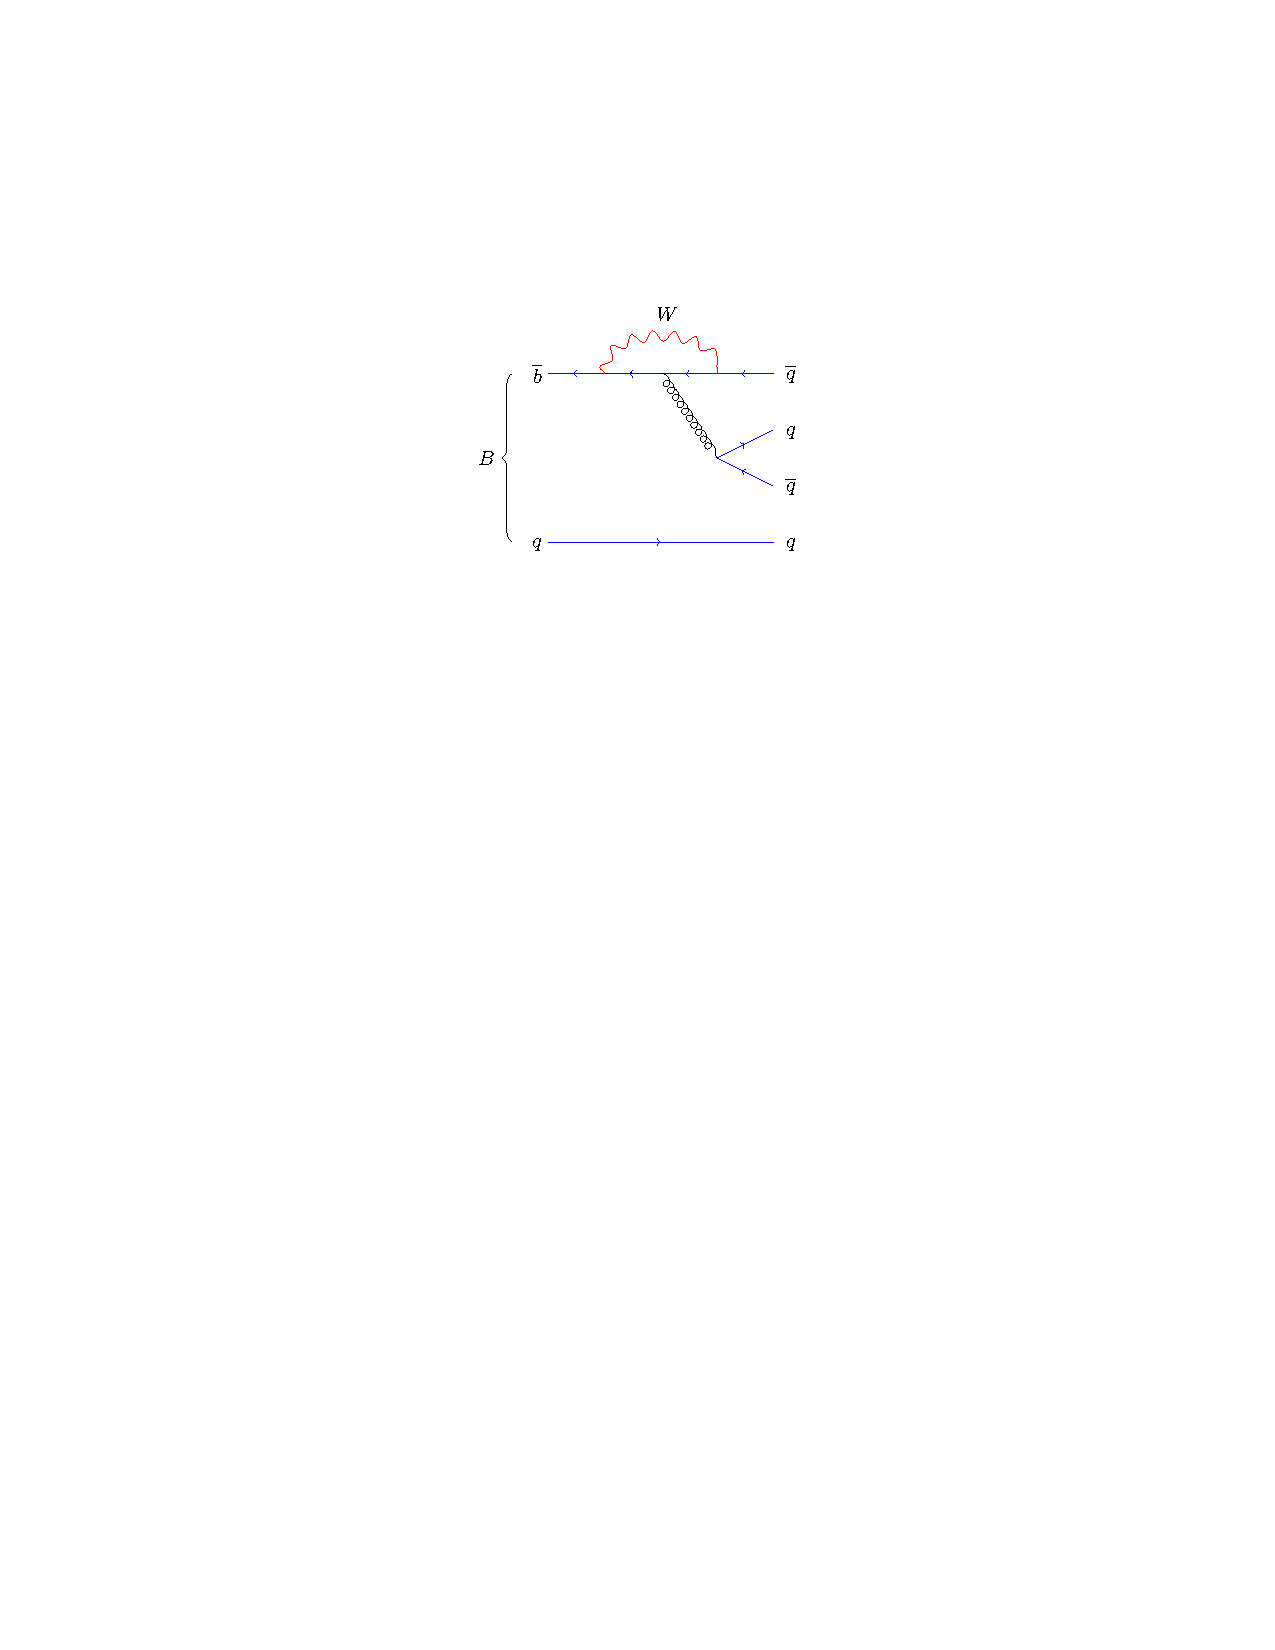
\includegraphics[width=1.0\textwidth]{figs/Theory/Peng.pdf}
        \caption{Penguin}
        \label{fig:theory_penguin}
    \end{subfigure}
    \begin{subfigure}[b]{0.32\textwidth}
        \centering
        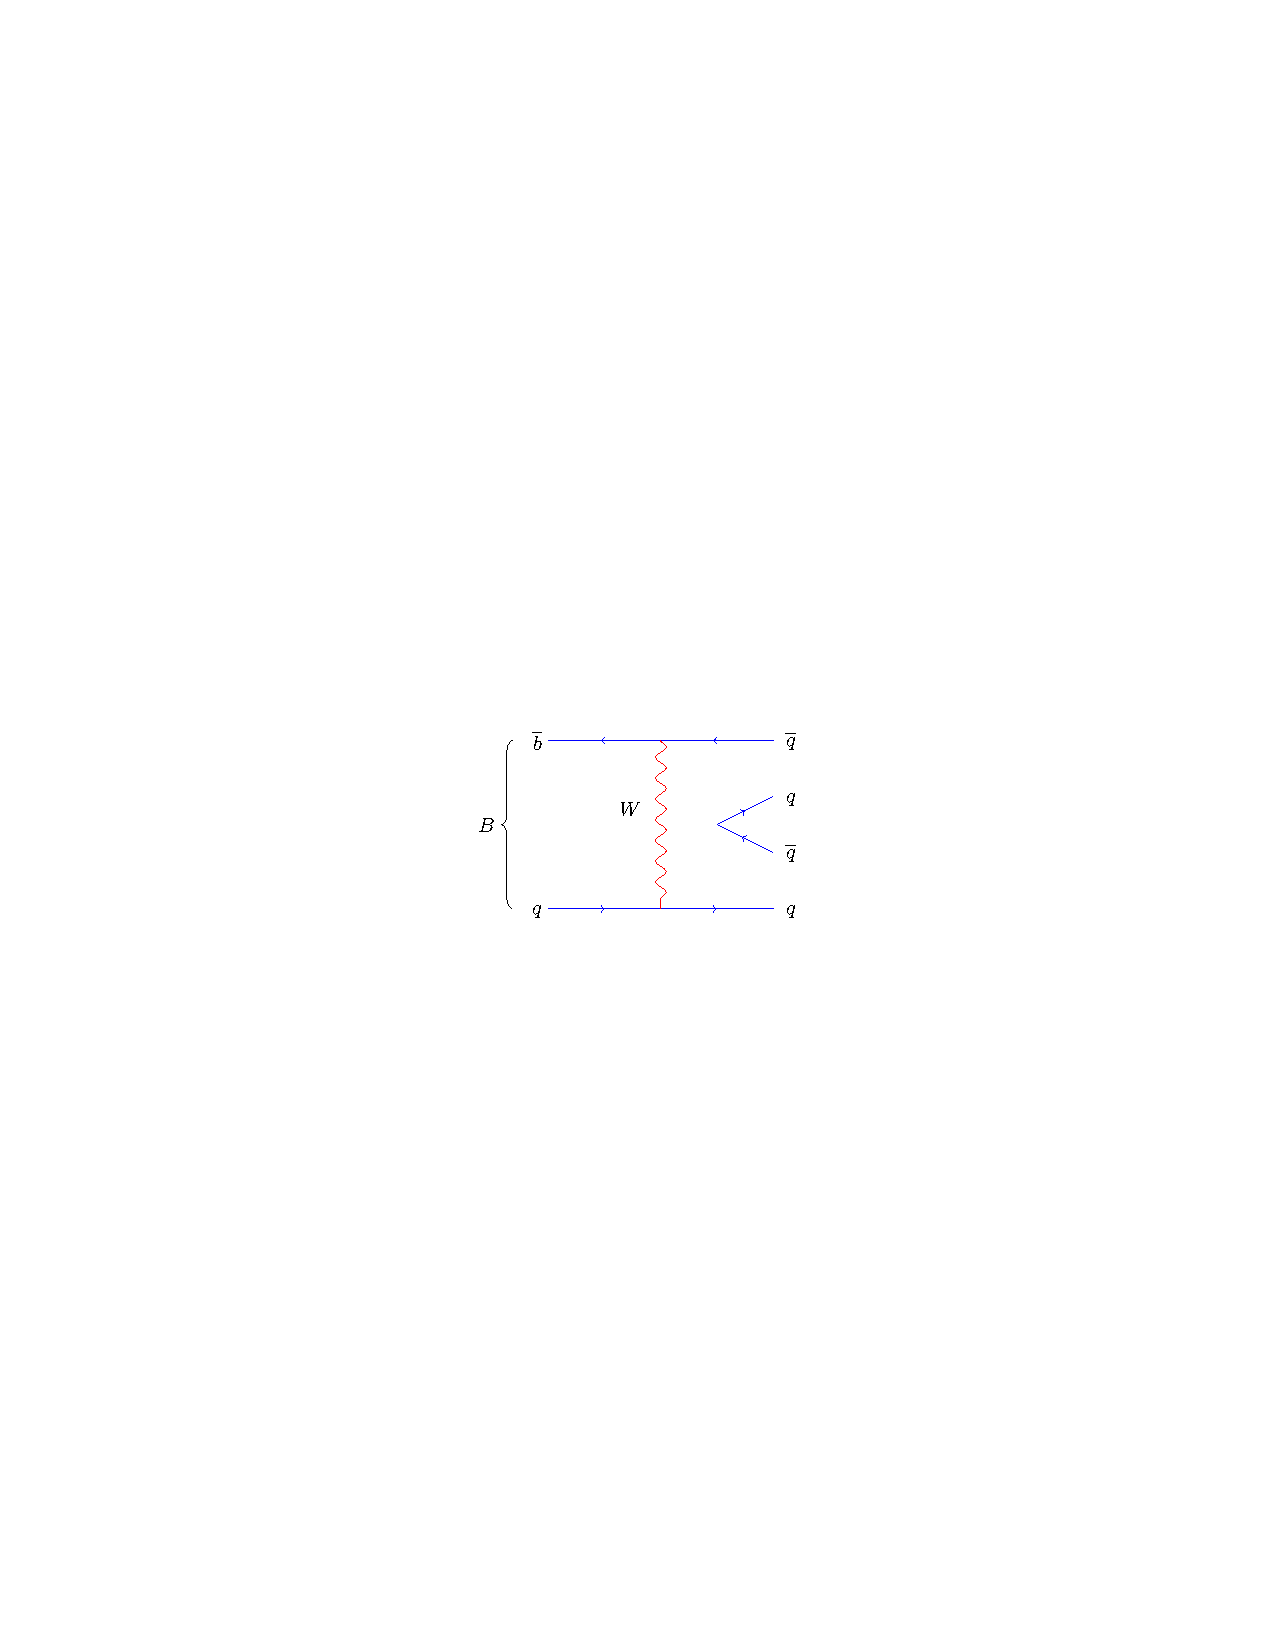
\includegraphics[width=1.0\textwidth]{figs/Theory/Exch.pdf}
        \caption{\W-boson exchange}
        \label{fig:theory_exchange}
    \end{subfigure}
    \begin{subfigure}[b]{0.32\textwidth}
        \centering
        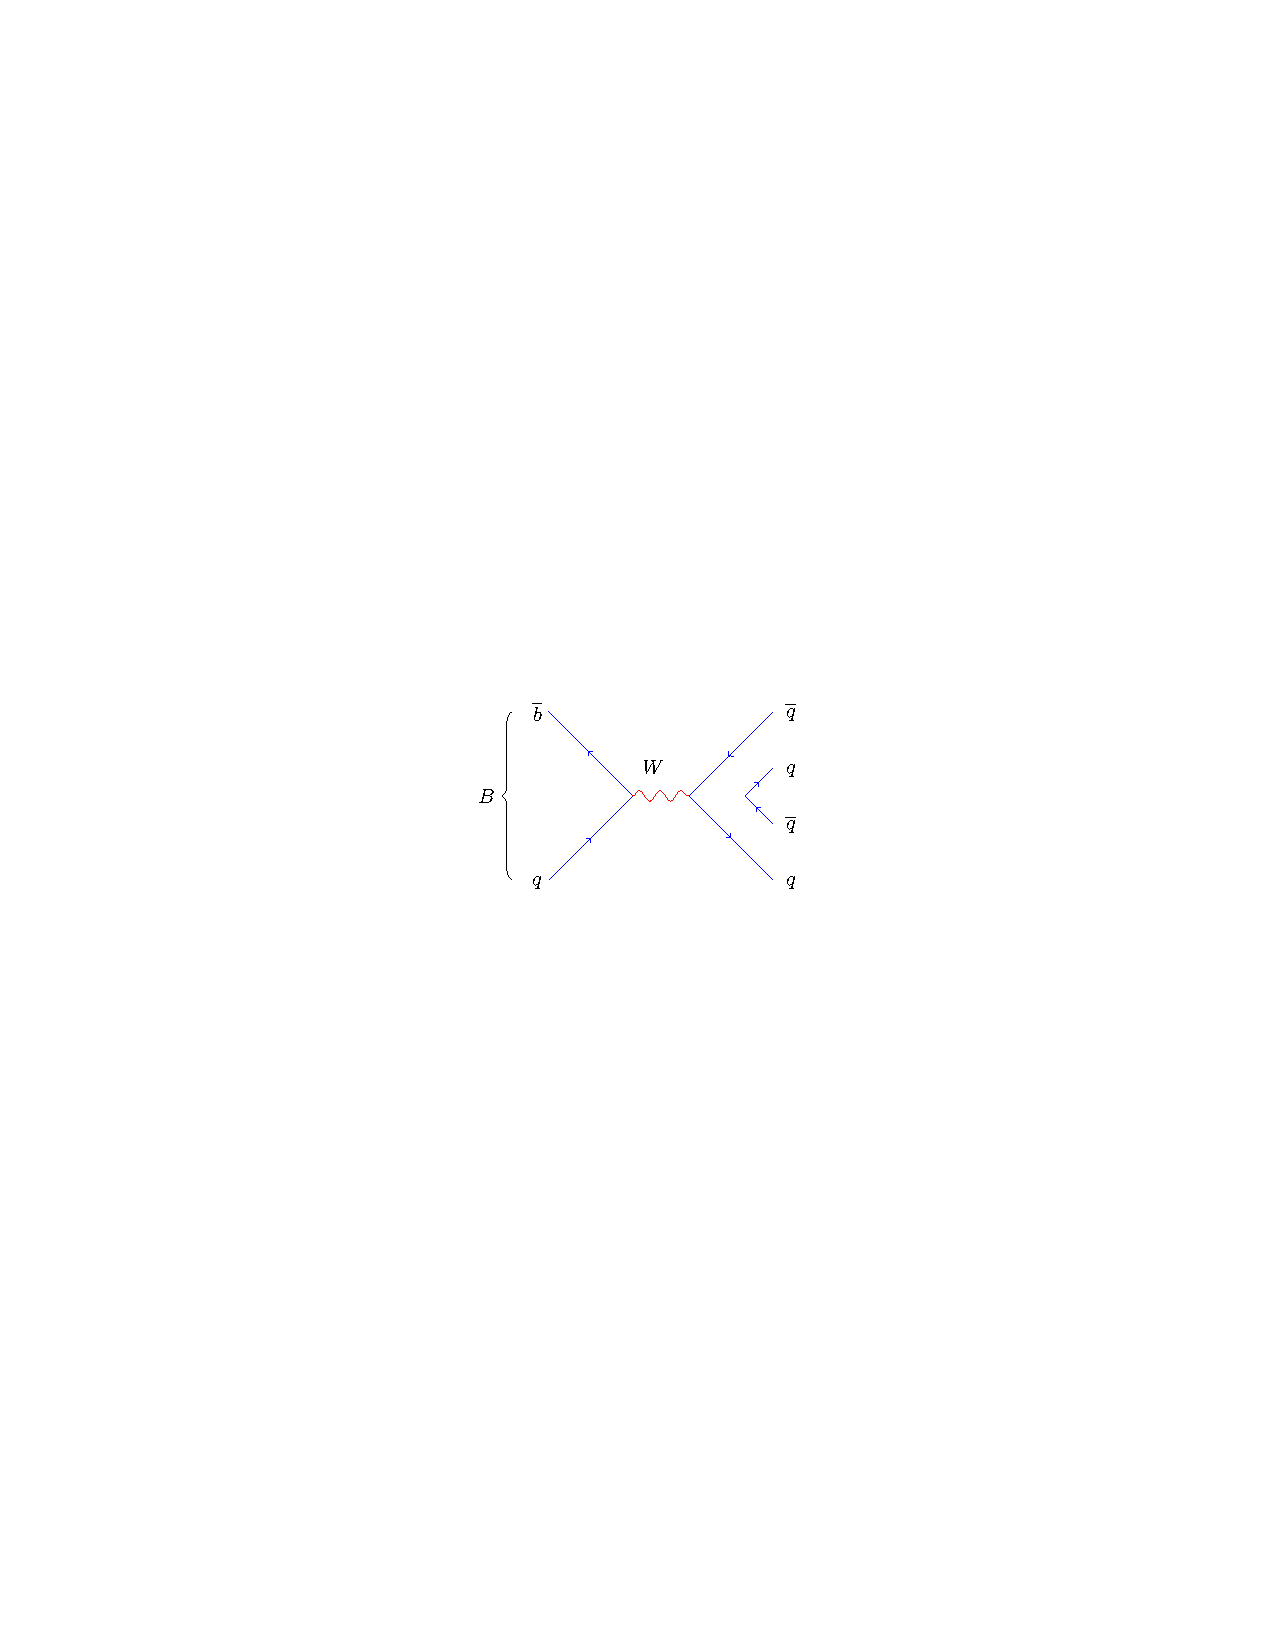
\includegraphics[width=1.0\textwidth]{figs/Theory/An.pdf}
        \caption{Annihilation}
        \label{fig:theory_ann}
    \end{subfigure}
    \begin{subfigure}[b]{0.32\textwidth}
        \centering
        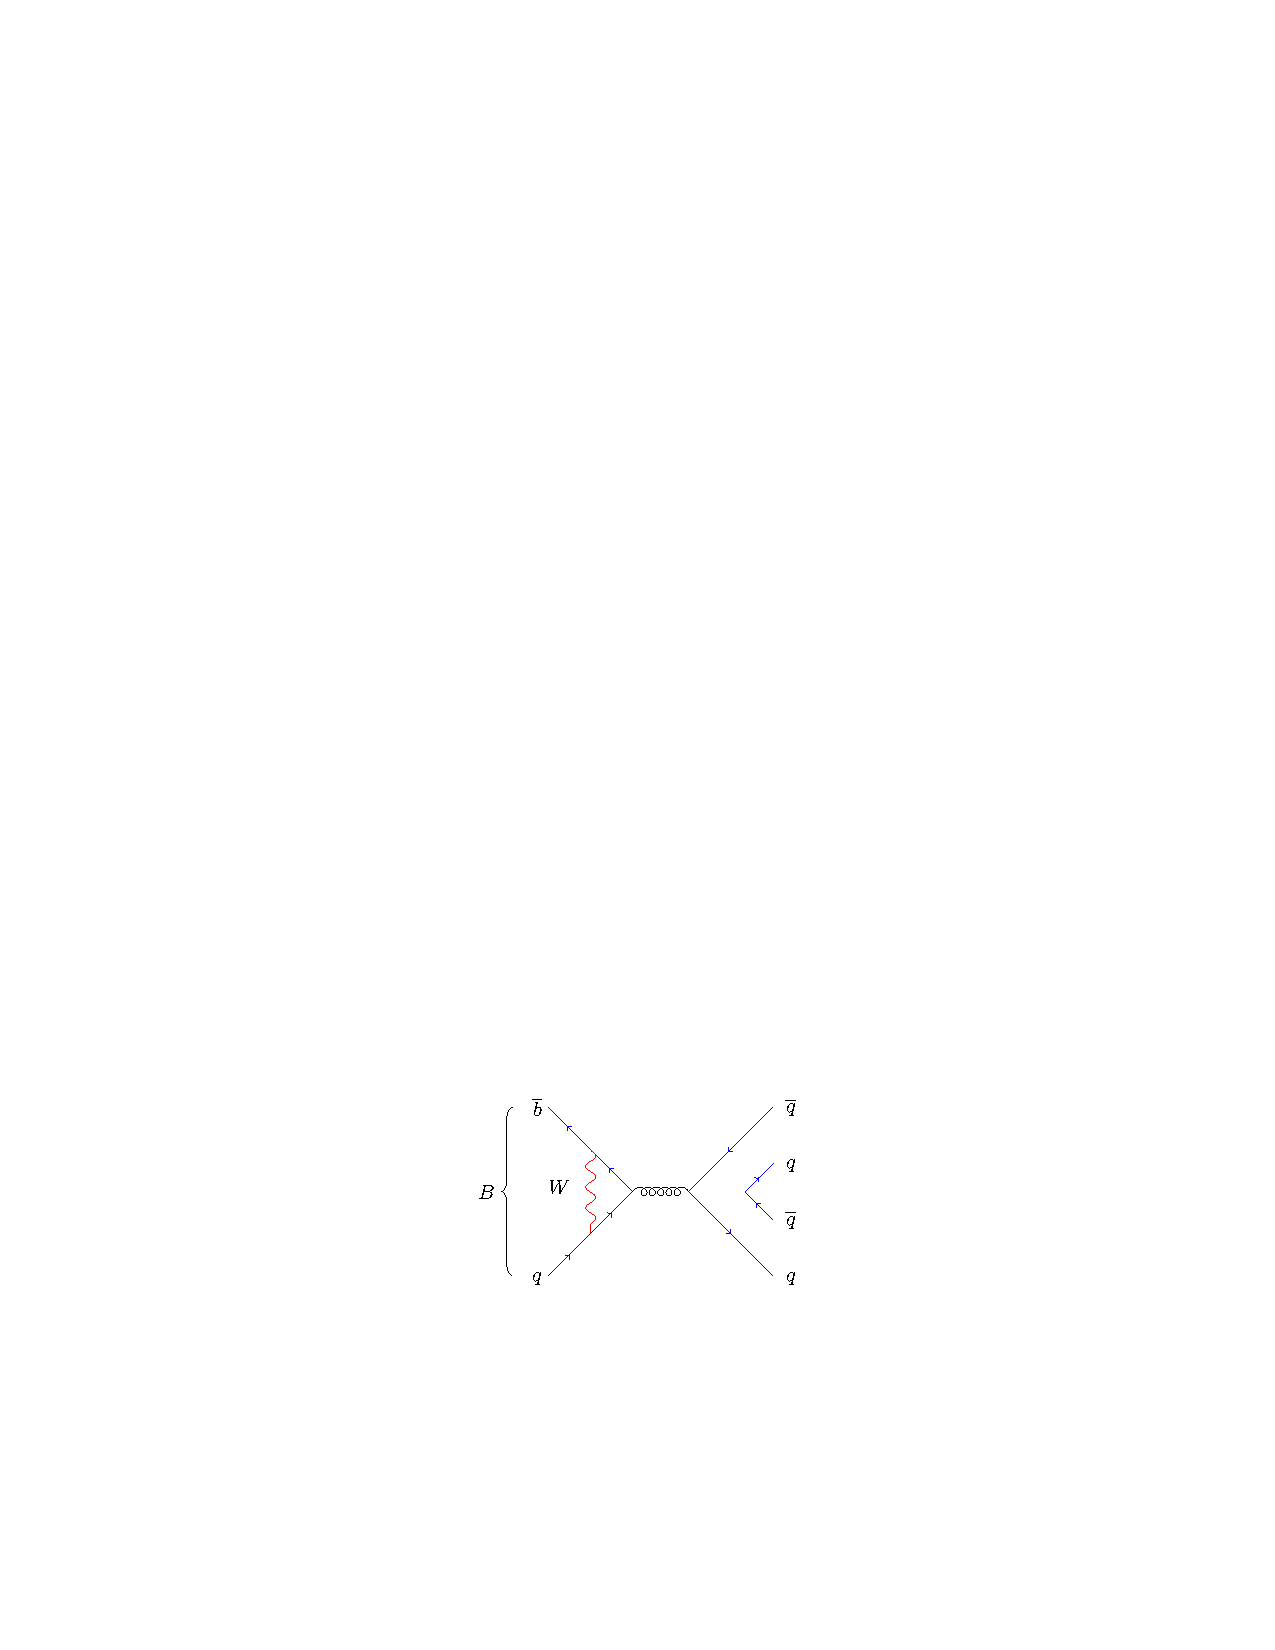
\includegraphics[width=1.0\textwidth]{figs/Theory/PengAn.pdf}
        \caption{Penguin Annihilation}
        \label{fig:theory_peng_ann}
    \end{subfigure}
    \caption{Two-body weak decay topologies of \bquark-mesons.}
    \label{fig:Theory_topo}   
\end{figure}
%%%%%%%%%%%%%%%%%%%%%%%%%%%%%%%%%%%%%%%%%%%%%%%%%%%%%%%%%%
These topologies receive varying levels of suppression as a result of the arrangement. The quark accompanying the \bquark-quark can act as a spectator (as in Figs.~\ref{fig:theory_colour_fav},~\ref{fig:theory_colour_sup}, and~\ref{fig:theory_penguin}) or can be involved in the decay process (as in Figs.~\ref{fig:theory_exchange},~\ref{fig:theory_ann},~\ref{fig:theory_peng_ann}).   



\subsection{QCD and hadronisation}

At low energies the weak interaction is weaker than electromagnetic and strong interactions, therefore weak processes can only be observed when electromagnetic and strong interactions are explicitly forbidden. Decays of ground state \Bp mesons are ideal as the flavour changing transitions can only be mediated by the weak interaction. In hadronic decays of \Bp mesons, the hadronisation of the final state still requires predictions from QCD.

At low energies QCD cannot be treated perturbatively as the coupling of the strong force remains large~\cite{PhysRevLett.30.1343,PhysRevLett.30.1346}. This means a large number of terms must be considered when calculating quantities. 
Various schemes are used to make these calculations more feasible: perturbation QCD can be performed at high energies; Lattice QCD in which space time is quantised; or various effective field theories.  
 
% {\color{Red}
% \begin{itemize}
% \item Explain why predictions are hard
% \item lattice QCD
% \item light cone sum rules? 
% \end{itemize}}

\section{Annihilation topology decays}

Annihilation topology decays are a class of processes in which the initial state particles annihilate to form a virtual propagator (Fig.~\ref{fig:theory_ann}). This mediator then decays to a (possibly different) set of particles.
Perhaps the simplest \Bp meson annihilation process is \decay{\Bp}{\ellp\neul}, shown in Fig.~\ref{fig:Theory_B2ellnu}. 
%%%%%%%%%%%%%%%%%%%%%%%%%%%%%%%%%%%%%%%%%%%%%%%%%%%%%%%%%%
\begin{figure}[!h]
    \centering
        \centering
        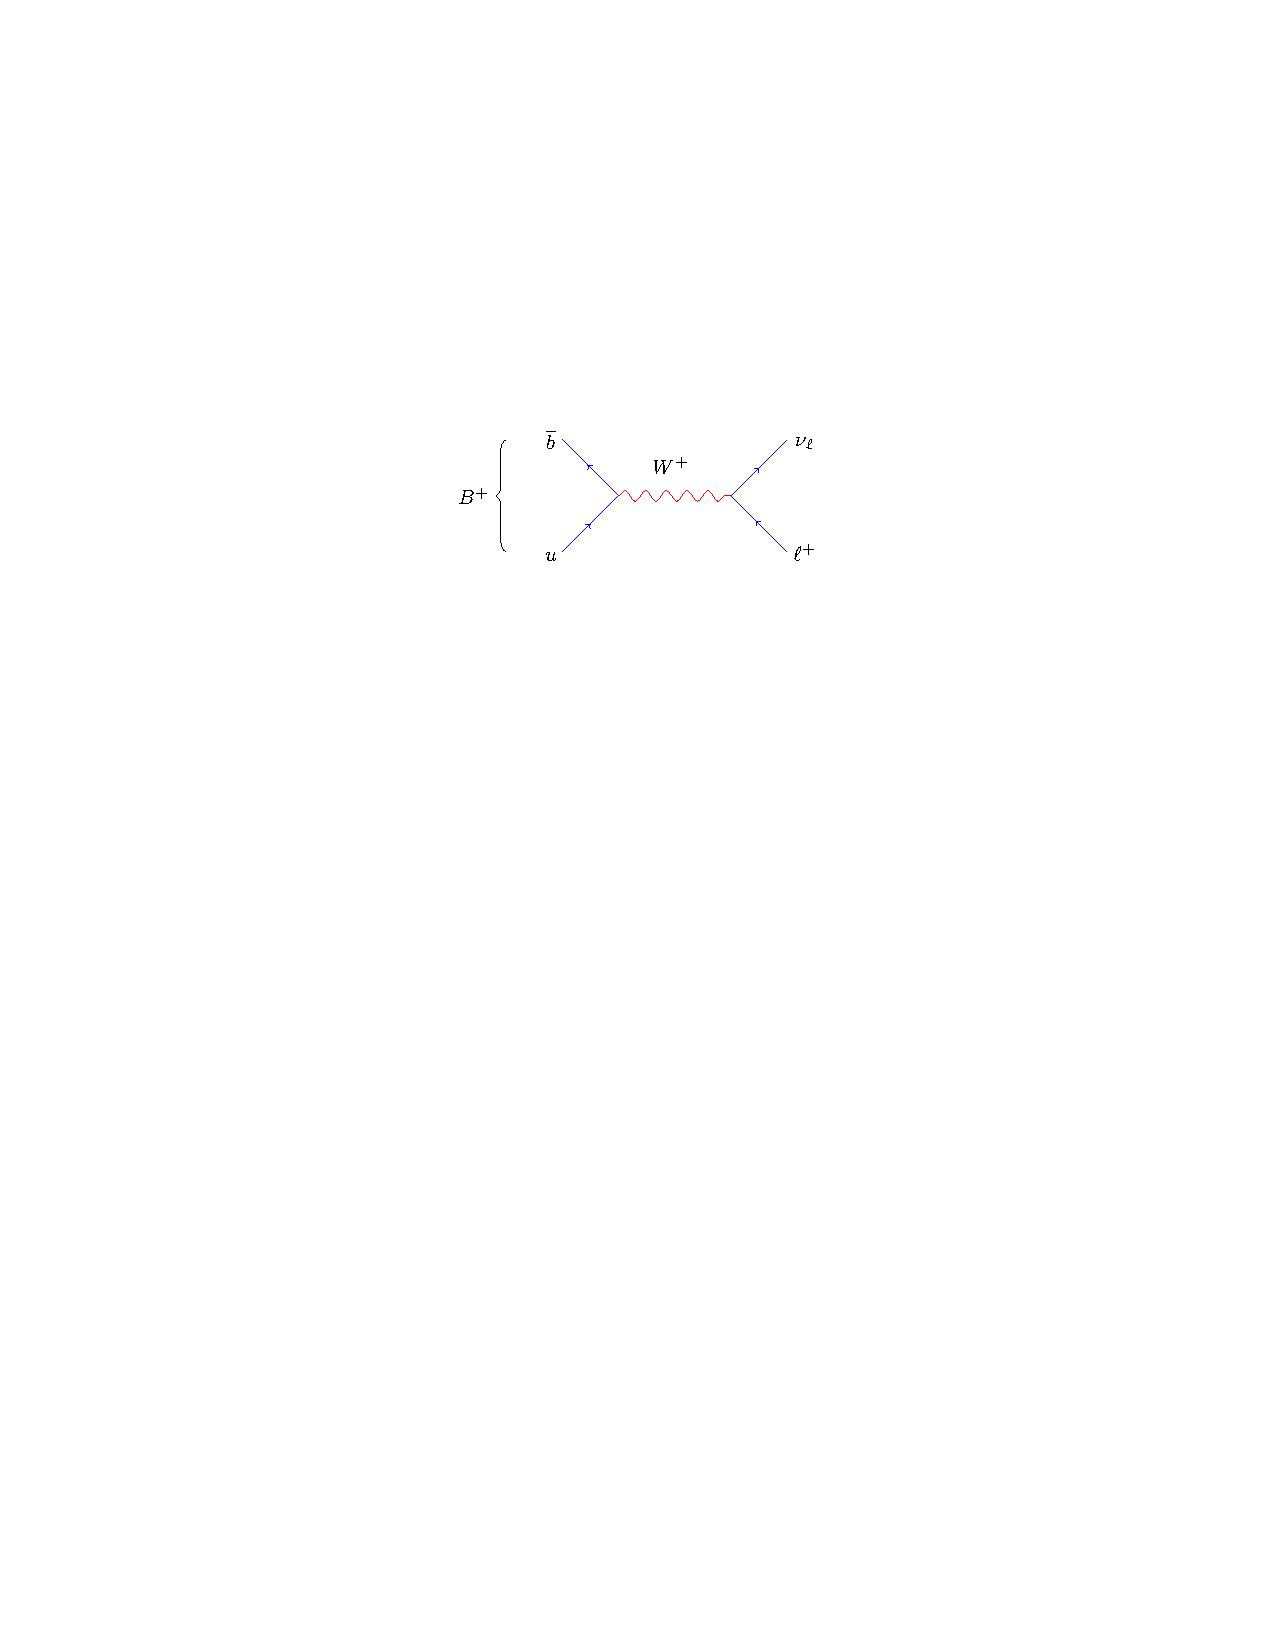
\includegraphics[width=0.5\textwidth]{figs/Theory/B2ellnu.pdf}
    \caption{Annihilation topology process for \decay{\Bp}{\ellp\neul} decays.}
    \label{fig:Theory_B2ellnu}   
\end{figure}
%%%%%%%%%%%%%%%%%%%%%%%%%%%%%%%%%%%%%%%%%%%%%%%%%%%%%%%%%%

\begin{table}[h]
   \begin{center}
      \begin{tabular}{lcc}
         \hline

         Decay Mode                 & SM prediction & Measurement \\
         \hline 
         \decay{\Bp}{\ep\neue}      & $(1.3\pm0.4)\times10^{-11}$           & $<9.8\times10^{-7}$\\
         \decay{\Bp}{\mup\neum}     & $(5.6\pm0.4)\times10^{-7}$            & $<1.0\times10^{-6}$\\
         \decay{\Bp}{\taup\neut}    & $(1.6\pm0.4)\times10^{-4}$&           $(1.09\pm0.24)\times 10^{-4}$ \\
         \hline
      \end{tabular}
   \end{center}
   \caption{Theoretical predictions and experimental measurements for \decay{\Bp}{\ellp\neul} processes, from Refs.~\cite{PhysRevD.92.051102,PhysRevD.79.091101,SATOYAMA200767}.}
   \label{tab:Theory_B2ellnu}
\end{table}
This purely leptonic \Bp meson decay can proceed to either of the three generations with the branching fractions detailed in Table~\ref{tab:Theory_B2ellnu}. The effect of helicity suppression in the final state is illustrated by the rapid decrease in predicted branching fraction as the mass charged lepton decreases. The neutrino in the final state makes this decay experimentally challenging to reconstruct at hadron colliders such as the \lhc. The measurement of \decay{\Bp}{\taup\neut} was performed at the \belle experiment, a \B-factory colliding \ep\en pairs at the $\PUpsilon(\text{4S})$ resonance. 
Hadronic annihilation decays are necessarily more complicated than these purely leptionic processes as the quark and antiquark must be further hadronised.

Decays that proceed via annihilation amplitudes are important in sectors other than \Bp decays. 

{\color{Red}
\begin{itemize}
\item Talk about \D and other annihilation topologies 
% \item Find origin of hadronic uncertainties 
\item \decay{\Bz}{\Kp\Km}? penguin annihilation
\item non pure - donals Bc
\end{itemize}}

\subsection{Pure annihilation topology decays}
Pure annihilation topology decays are an interesting subset of processes in which (at lowest order) only annihilation decay diagrams contribute. These are of particular interest because this allows the magnitudes of these processes to be isolated. Additionally, they provide a suitable forum in which to search for new physics; enhanced or decreased branching fractions and non-zero \CP violations are symptomatic of multiple competing processes interfering with one another.  

Typically, hadronic \emph{pure} annihilation processes are characterised by a mutually exclusive set of quarks in the initial and final state. This implies that the initial state must have completely annihilated into a mediator for this process to occur.   

In the \Bp sector two decays are of particular interest; \decay{\Bp}{\Dsp\phiz} and \decay{\Bp}{\Dp\Kstarz}.

Pure anihliation decays are also of particular interest in the \Bc sector. Charmless decays of \Bcp mesons can proceed exclusively via annihilation topologies~\cite{PhysRevD.80.114031}. These additionally benefit from the larger size of the CKM matrix element \Vcb with respect to \Vub.


\section{Rescattering}

Rescattering allows \Bp mesons to decay to final states that are ideal pure annihilation topologies via an intermediate process of some other topology. This can potential limit the sensitivity the annihilation decay if these processes happen at a significant rate. Intermediate processes that could contribute to the \decay{\Bp}{\Dsp\phiz} decay are shown in Fig.~\ref{fig:Theory_rescattering}~\cite{Gronau:2012gs}. These rather complicated processes both involve tree-level \decay{\bquarkbar}{\uquarkbar} transitions in which one of both of the products undergo a final state interactions.  

%%%%%%%%%%%%%%%%%%%%%%%%%%%%%%%%%%%%%%%%%%%%%%%%%%%%%%%%%%
\begin{figure}[!h]
    \centering
    \begin{subfigure}[m]{0.7\textwidth}
        \centering
        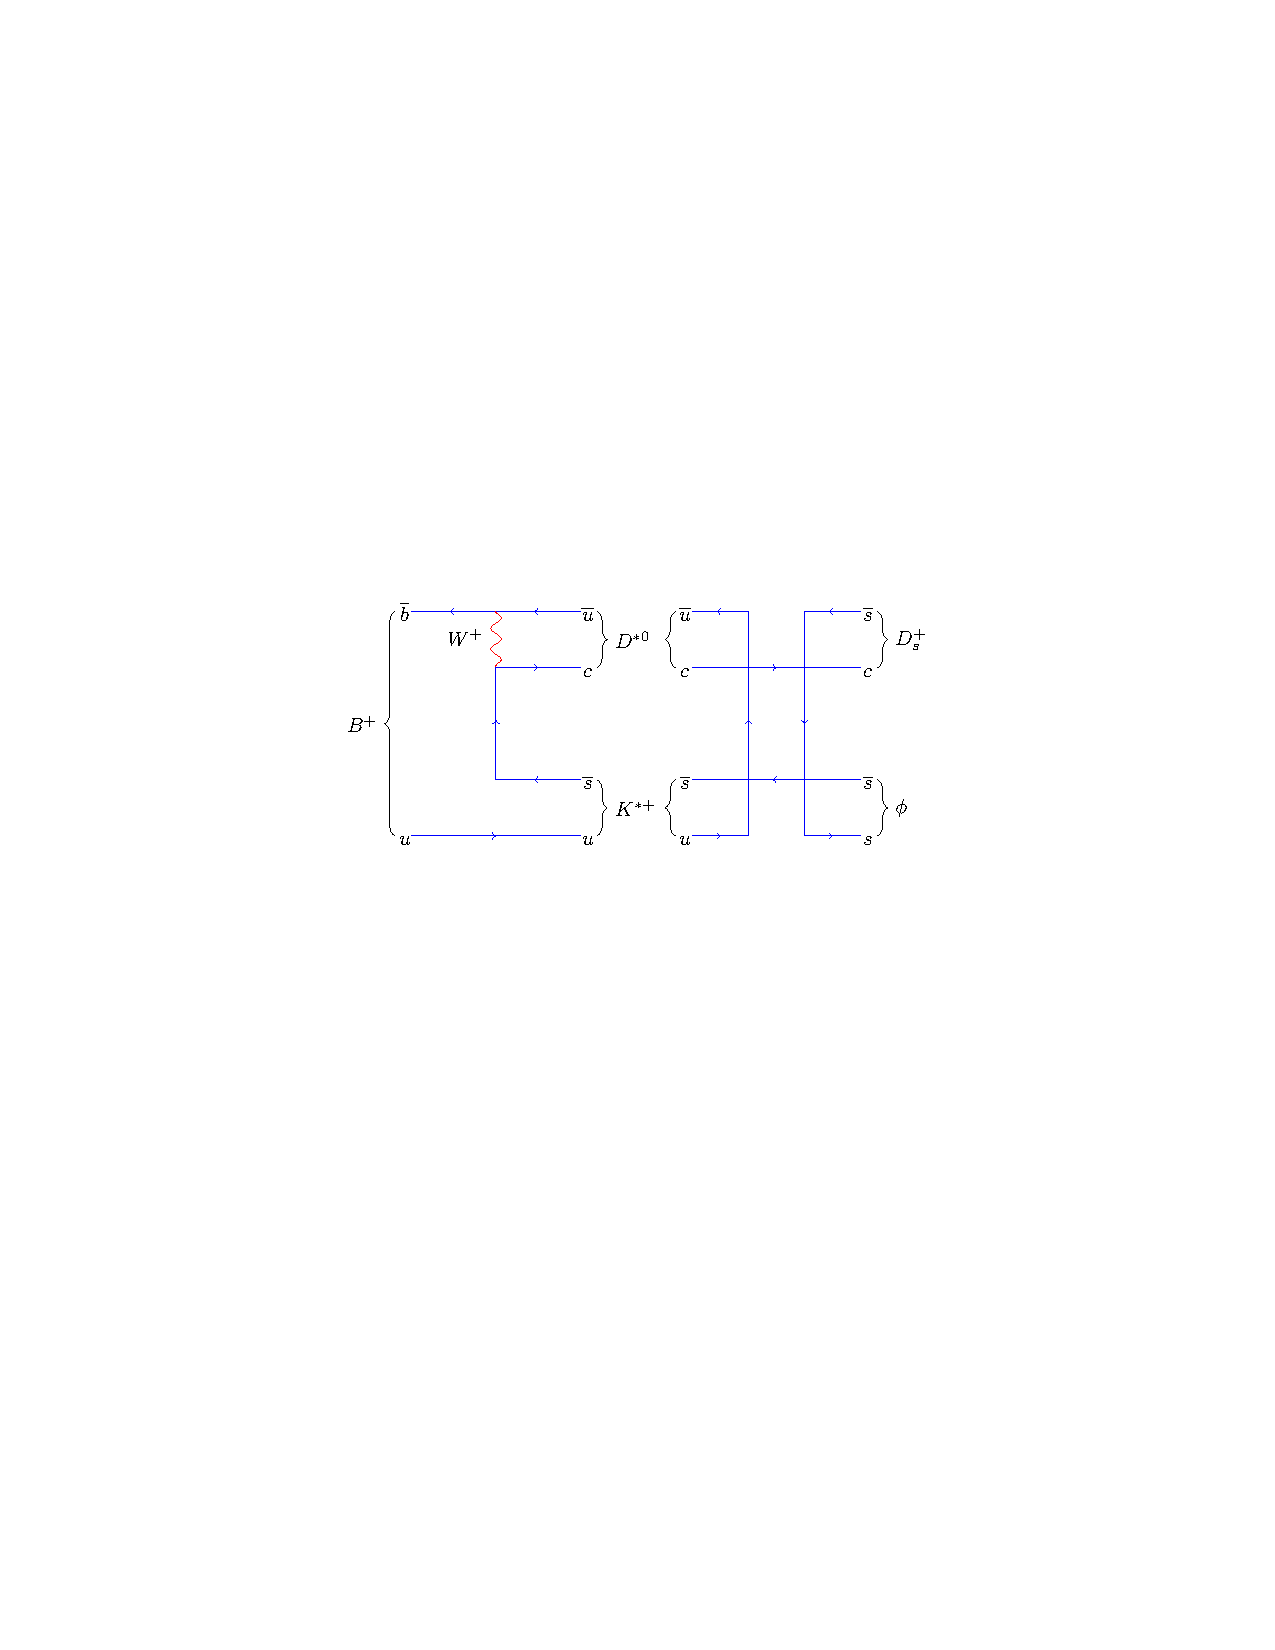
\includegraphics[width=1.0\textwidth]{figs/Theory/B2DsPhi_Rescattering_B2D0K.pdf}
        \caption{via \decay{\Bp}{\Dstarz\Kstarp}}
        \label{fig:theory_rescattering_DK}
    \end{subfigure}
    \begin{subfigure}[m]{0.7\textwidth}
        \centering
        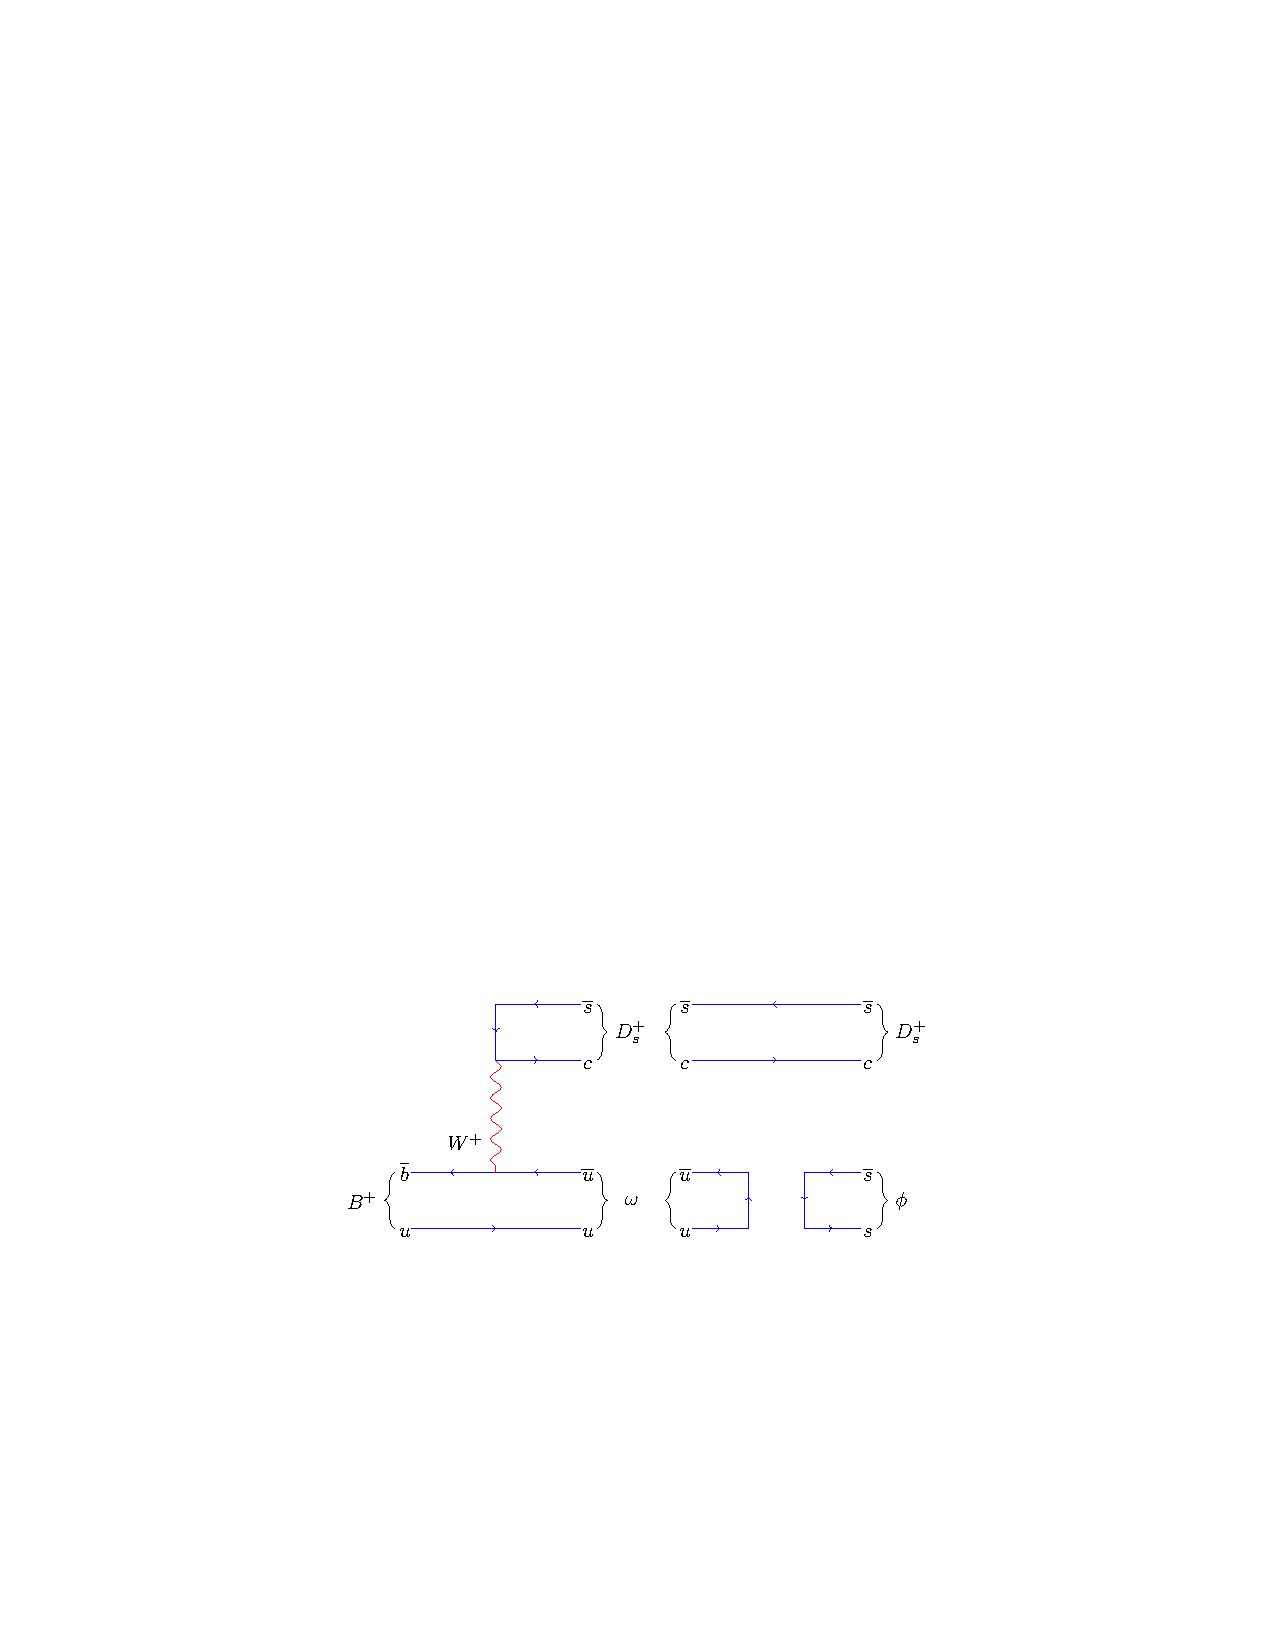
\includegraphics[width=1.0\textwidth]{figs/Theory/B2DsPhi_Rescattering_B2Dsomega.pdf}
        \caption{via $\decay{\Bp}{\Dsp\omega}$}
        \label{fig:theory_rescattering_DsO}
    \end{subfigure}
    \caption{Rescattering contributions to \decay{\Bp}{\Dsp\phiz} decays.}
    \label{fig:Theory_rescattering}   
\end{figure}
%%%%%%%%%%%%%%%%%%%%%%%%%%%%%%%%%%%%%%%%%%%%%%%%%%%%%%%%%%
In Fig.~\ref{fig:theory_rescattering_DK}, the path via the \decay{\Bp}{\Dstarz\Kstarp} intermediate state is shown. The initial process is a weak colour-suppressed tree level decay, followed by a strong final state interaction that interchanges the quark flavours. 

An alternative path via the state $\decay{\Bp}{\Dsp\omega}$ is shown in Fig.~\ref{fig:theory_rescattering_DsO}. This is a colour-favoured tree level process followed by the mixing of a $\omega$ meson to a \phiz meson. This $\omega-\phi$ mixing has been shown to be small as a result of OZI suppression~\cite{OKUBO1963165,PhysRevD.79.074006}.


% {\color{Red}
% \begin{itemize}
% \item What is rescattering?
% \item Examples of it?
% \item Why it's expected to be small
% \item $\decay{\Bu}{\Dsp\omega}$
% \item $\omega\to\phi$ is OZI suppressed 
% \item $\decay{\Bu}{\Dz\Kstarp}$
% \item References: \Dp\Kstarz~\cite{Mehraban2016}.
% \item $\omega - \phi$ mixing: ~\cite{OKUBO1963165,PhysRevD.79.074006}.
% \end{itemize}}

\section{Theoretical predictions for the \decay{\Bp}{\Dsp\phiz} decay}

%%%%%%%%%%%%%%%%%%%%%%%%%%%%%%%%%%%%%%%%%%%%%%%%%%%%%%%%%%
\begin{figure}[!h]
    \centering
    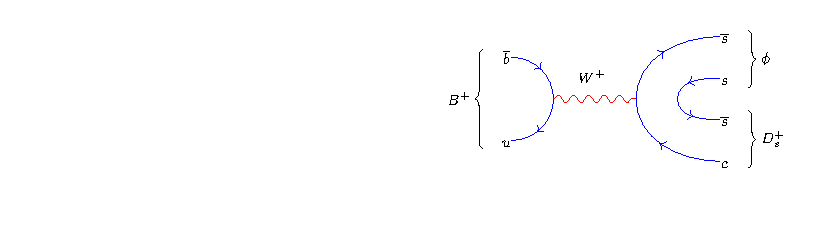
\includegraphics[width=0.6\textwidth]{figs/Theory/B2DsPhi.pdf}
    \caption{\decay{\Bp}{\Dsp\phiz} }
    \label{fig:Theory_DsPhiDiagram}   
\end{figure}
%%%%%%%%%%%%%%%%%%%%%%%%%%%%%%%%%%%%%%%%%%%%%%%%%%%%%%%%%%



{\color{Blue}
In the SM, the decay $\decay{\Bp}{\Dsp\phi}$ proceeds dominantly via the annihilation diagram shown in Fig.~\ref{fig:Theory_DsPhiDiagram}. 
This suppressed topology requires the wave functions of the incoming quarks to overlap sufficiently to annihilate into a virtual \Wp boson. 
The decay is further suppressed by the small magnitude of the CKM matrix element \Vub associated with the annihilation vertex. 


}

\subsection{Standard model predictions}
{\color{Blue}
Several SM predictions have been made for the branching fraction of the $\decay{\Bp}{\Dsp\phi}$ decay~\cite{Zou:2009zza, Mohanta:2002wf, Mohanta:2007uu, Lu:2001yz}, using input from lattice calculations~\cite{fB:2013HPQCD,fB:2016ETM, fB:2016Fermi}. These predictions are in the range $(1-7)\times10^{-7}$, where the limit on the precision is dominated by hadronic uncertainties. 

In addition, unlike many rare hadronic decays including $\decay{\Bp}{\Dsp\Kp\Km}$, possible contributions from rescattering effects are expected to be small, for example contributions from intermediate states such as $\decay{\Bp}{\Dsp\omega}$~\cite{Gronau:2012gs}.

}

{\color{Red}
\begin{itemize}
\item Find origin of hadronic uncertainties 
\end{itemize}}

\subsection{BSM models and predictions}
{\color{Blue}
However, additional diagrams contributing to this decay can arise in some extensions of the SM, such as supersymmetric models with R-parity 
violation. They could enhance the branching fraction and/or produce large \CP asymmetries~\cite{Mohanta:2002wf, Mohanta:2007uu}, which makes the $\decay{\Bp}{\Dsp\phi}$ decay a promising place to search for new physics beyond the SM.\footnote{Charge conjugation is implied throughout this paper. Furthermore, $\phi$ denotes the $\phi(1020)$ resonance.}
}

{\color{Red}
\begin{itemize}
\item Higgs doublet
\item SUSY 
\item include feynman diagrams
\item small intro into models
\end{itemize}}

\subsection{Previous measurements}

{\color{Blue}
The \lhcb experiment reported evidence for the decay $\decay{\Bp}{\Dsp\phi}$ using $pp$ collision data corresponding to an integrated luminosity of 1\invfb taken during 2011, at a centre-of-mass energy of 7\tev~\cite{Aaij:2012zh}. A total of $6.7^{+4.5}_{-2.6}$ candidates was observed. The branching fraction was determined to be 

\begin{equation}
\mathcal{B}(\decay{\Bp}{\Dsp\phi}) = (1.87^{+1.25}_{-0.73} \pm 0.19 \pm 0.32) \times 10^{-6},
\end{equation}
where the first uncertainty is statistical, the second is systematic and the third is due to the uncertainty on the branching fraction of the decay $\decay{\Bp}{\Dsp\Dzb}$, which was used as normalisation. 
Given the large uncertainties on both the theoretical and experimental values, the previously measured value is consistent with the range of SM values given above.
}

{\color{Red}
\begin{itemize}
\item Include plot and measurement
\item say something about similarites 
\end{itemize}}


\section{Theoretical predictions for the \decay{\Bp}{\Dsp\Kp\Km} decay}


%%%%%%%%%%%%%%%%%%%%%%%%%%%%%%%%%%%%%%%%%%%%%%%%%%%%%%%%%%
\begin{figure}[!h]
    \centering
    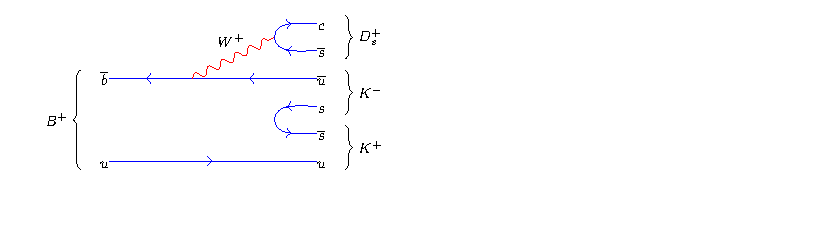
\includegraphics[width=0.6\textwidth]{figs/Theory/B2DsKK.pdf}
    \caption{\decay{\Bp}{\Dsp\Kp\Km} }
    \label{fig:Theory_DsKKDiagram}   
\end{figure}
%%%%%%%%%%%%%%%%%%%%%%%%%%%%%%%%%%%%%%%%%%%%%%%%%%%%%%%%%%



{\color{Blue}
The decay $\decay{\Bp}{\Dsp\Kp\Km}$ is mediated by a $\decay{\bquarkbar}{\uquarkbar}$ transition shown in Fig.~\ref{fig:Theory_DsKKDiagram} and is therefore suppressed in the Standard Model (SM) due to the small size of the Cabibbo-Kobayashi-Maskawa (CKM) matrix element \Vub. 
}


{\color{Red}
\begin{itemize}
\item explain what a dalitz plot is
\end{itemize}
}

\subsection{Standard model predictions}
{\color{Blue}
The branching fraction for this decay is currently not measured, however a similar decay, \decay{\Bp}{\Dsp \piz}, has been observed with a branching fraction of $\mathcal{B}(\decay{\Bp}{\Dsp \piz}) = (1.5 \pm 0.5) \times 10^{-5}$~\cite{Aubert:2006xy}.
}


{\color{Red}
\begin{itemize}
\item talk about \decay{\Bp}{\Dsp\piz}
\item Could talk about \decay{\Bp}{\Dp\Kp\pim} and estimate   
\end{itemize}}

\subsection{Previous measurements}



